\documentclass[16pt,norsk,a4paper]{article}
\usepackage[utf8]{inputenc}
\usepackage[T1]{fontenc}
\usepackage[norsk]{babel}
\usepackage[cm]{fullpage}
\usepackage{color}
\usepackage{parskip,textcomp,amssymb,graphicx}
\usepackage{pdfpages}

\title{Generalforsamling\\
	Høst 2015\\
	Cybernetisk Selskab\\[.3cm]
	
\includegraphics[width=0.4\textwidth]{cyblogoa3.pdf}\\[-.8cm]}
\date{19. nov 2015}

\begin{document}
\maketitle{}
\newpage
\tableofcontents{}

%\newpage
~\\

\section{Valg av møteleder}

\section{Valg av referent}

\section{Valg av protokollunderskrivere}

\section{Valg av tellekorps}

\section{Godkjenning av innkalling}

\section{Godkjenning av dagsorden}

\newpage


\section{Semesterberetninger}
\subsection{Semesterberetning ved Leder}
Driften dette semesteret har ikke skilt seg nevneverdig ut fra tidligere. Som før blir høstsemesteret dominert av fadderuka og dagen@ifi. I år klarte vi endelig å få til en kantinefest i løpet av fadderuka. Dette ble en suksess og jeg håper det blir gjentatt neste høst. Dagen@ifi ble gjennomført på en god måte og resultatet er veldig likt tidligere år. Andre arrangementer det er verdt å nevne er navet-kcikoff og flere andre arrangementer med navet, samt masterkickoff med dagen@ifi. I tillegg har vi tradisjonen tro avholdt whisky-seminar og flere andre kjente CYB-arrangementer.\\

Når det kommer til den vanlige driften så er det meste som før. Vi har sett en liten oppsving i rekruttering, spesielt til bar. Vi håper også dette vil føre til flere nye aktive skjenkemestre i semesteret som kommer.\\

Til slutt vil jeg takke for et flott semester og håper vi fortsetter å arbeide skikkelig med å holde CYB gående på en såpass god måte som vi gjør nå.\\

Til slutt vil jeg takke for et flott semester og håper vi fortsetter å arbeide skikkelig med å holde CYB gående på en såpass god måte som vi gjør nå.\\
\

Jan Kristian Furulund,\\
Leder Cybernetisk Selskab\\
Høst 2015

%\newpage


\subsection{Semesterberetning ved Kjellermogul}
Dette semesteret har det egentlig ikke skjedd så alt for mye utenom det normale,
personlig har jeg feildømt arbeidsmengden i denne studietingen Staten maser på at jeg er på Ifi for å gjennomføre.
Så har ikke til alle tider hatt nok tid til å følge opp alt jeg burde følge opp.\\

Videre så har vi oppgradert kortterminalene våre til trådløse. Taktiske som vi er introduserte vi dette til første dag i fadderukene, og det kunne nok fint gått bedre.
Endte med store mengder avvik pga uvante systemer, dette har tatt seg inn igjen gjennom semesteret og man er nå innenfor rimelige marginer.
Burde enda skjerpes inn enda mer på generelle rutiner i alle grupper, men håper det går bedre til våren hvor alle har blitt mer kjent med Escape.\\

Skiftfylling har gått strålende, spesielt i fadderukene hvor vi hadde tilnærmet ingen hull med unntak av ctrl-alt-del hvor grunnet brukerfeil vi måtte sende en
på legevakta og litt feilberegning i antall funker. Dette var til dels pga vi ga Internstatus til de som hadde tatt ett skift i samme stil som RF gjør.
Og til dels pga noen superfunker som stiller på alt for mye.\\

Nå som jeg forhåpentligvis blir ferdig med Bacheloren får jeg endelig nok tid til å gjennomføring av mine ønsker ovenfor Escape, som flere eventer i Escape
og forbedring av atmosfæren i lokale "overall".\\
\

Nikolas Papaioannou,\\
Kjellermogul Cybernetisk Selskab\\
Høst 2016

\newpage

\section{Regnskap vår 2015}
Kasserer orienterer om regnskapsrapporten for vår 2015. Henviser til vedlegg.\\

%\newpage

\section{budsjett 2016}
Kasserer orienterer om budsjett høst 2016. Henviser til vedlegg.\\

%\newpage

\section{Kontingentfastsettelse}
Hovedstyret foreslår å holde medlemskontigenten på 30 kroner.\\

\section{Valg}

\subsection{Hovedstyret}
Man velges inn i hovedstyret for ett år av gangen.

\subsubsection{Arrangementsjef}

\subsubsection{Kasserer}

\subsubsection{Promoteringsansvarlig}

\subsubsection{Internansvarlig}

\subsubsection{Rekruttering}

\subsection{Kjellerstyret}
Økonomiansvarlig velges for ett år av gangen, mens de resterende vervene velges for ett semester.
\subsubsection{Økonomiansvarlig}

\subsubsection{Barsjef}

\subsubsection{Kafésjef}

\subsubsection{DJ-sjef}

\subsubsection{Innkjøpsansvarlig}

\subsubsection{Teknisk ansvarlig}

\subsubsection{Utlånsansvarlig}

%\newpage

\section{Vedtektsendringer}

\subsection{§1 Tilhørighet og formål.}
Legge til en før instituttforening og endre for til ved\\
Gammel tekst:\
§1a) Cybernetisk Selskab er instituttforening for Institutt for informatikk ved Universitetet i Oslo.\\

Ny tekst:\
§1a) Cybernetisk Selskab er en instituttforening ved Institutt for informatikk ved Universitetet i Oslo.

\subsection{§5 Hovedstyret.}
Endre "men kun styremedlemmer har stemmerett" til "men kun styrets medlemmer har stemmerett"\\

Gammel tekst:\
§5f) Alle medlemmer i henhold til §2 har møterett på hovedstyrets møter, men kun styremedlemmer
har stemmerett.

Ny tekst:\
§5f) Alle medlemmer i henhold til §2 har møterett på hovedstyrets møter, men kun styrets medlemmer
har stemmerett.

\subsection{§6 Kjellerstyret.}
Legge til nytt punkt på slutten:
§6f) Alle medlemmer i henhold til §2 har møterett på kjellerstyrets møter, men kun styrets medlemmer har stemmerett.

\subsection{§10 Oppløsning}
Endre aktiva til medler og endre IFI til ifi

Gammel tekst:
§10c) Dersom foreningen oppløses, går foreningens aktiva til Fordelingsutvalget (FU) ved Institutt for
informatikk (IFI).

Ny tekst:\
§10c) Dersom foreningen oppløses, går foreningens midler til Fordelingsutvalget (FU) ved Institutt for
informatikk (Ifi).


\section{Utdeling av pins}
Mats Astrup Scjølberg deler ut pins.\\

\newpage

\section*{Vedlegg: Vedtekter}

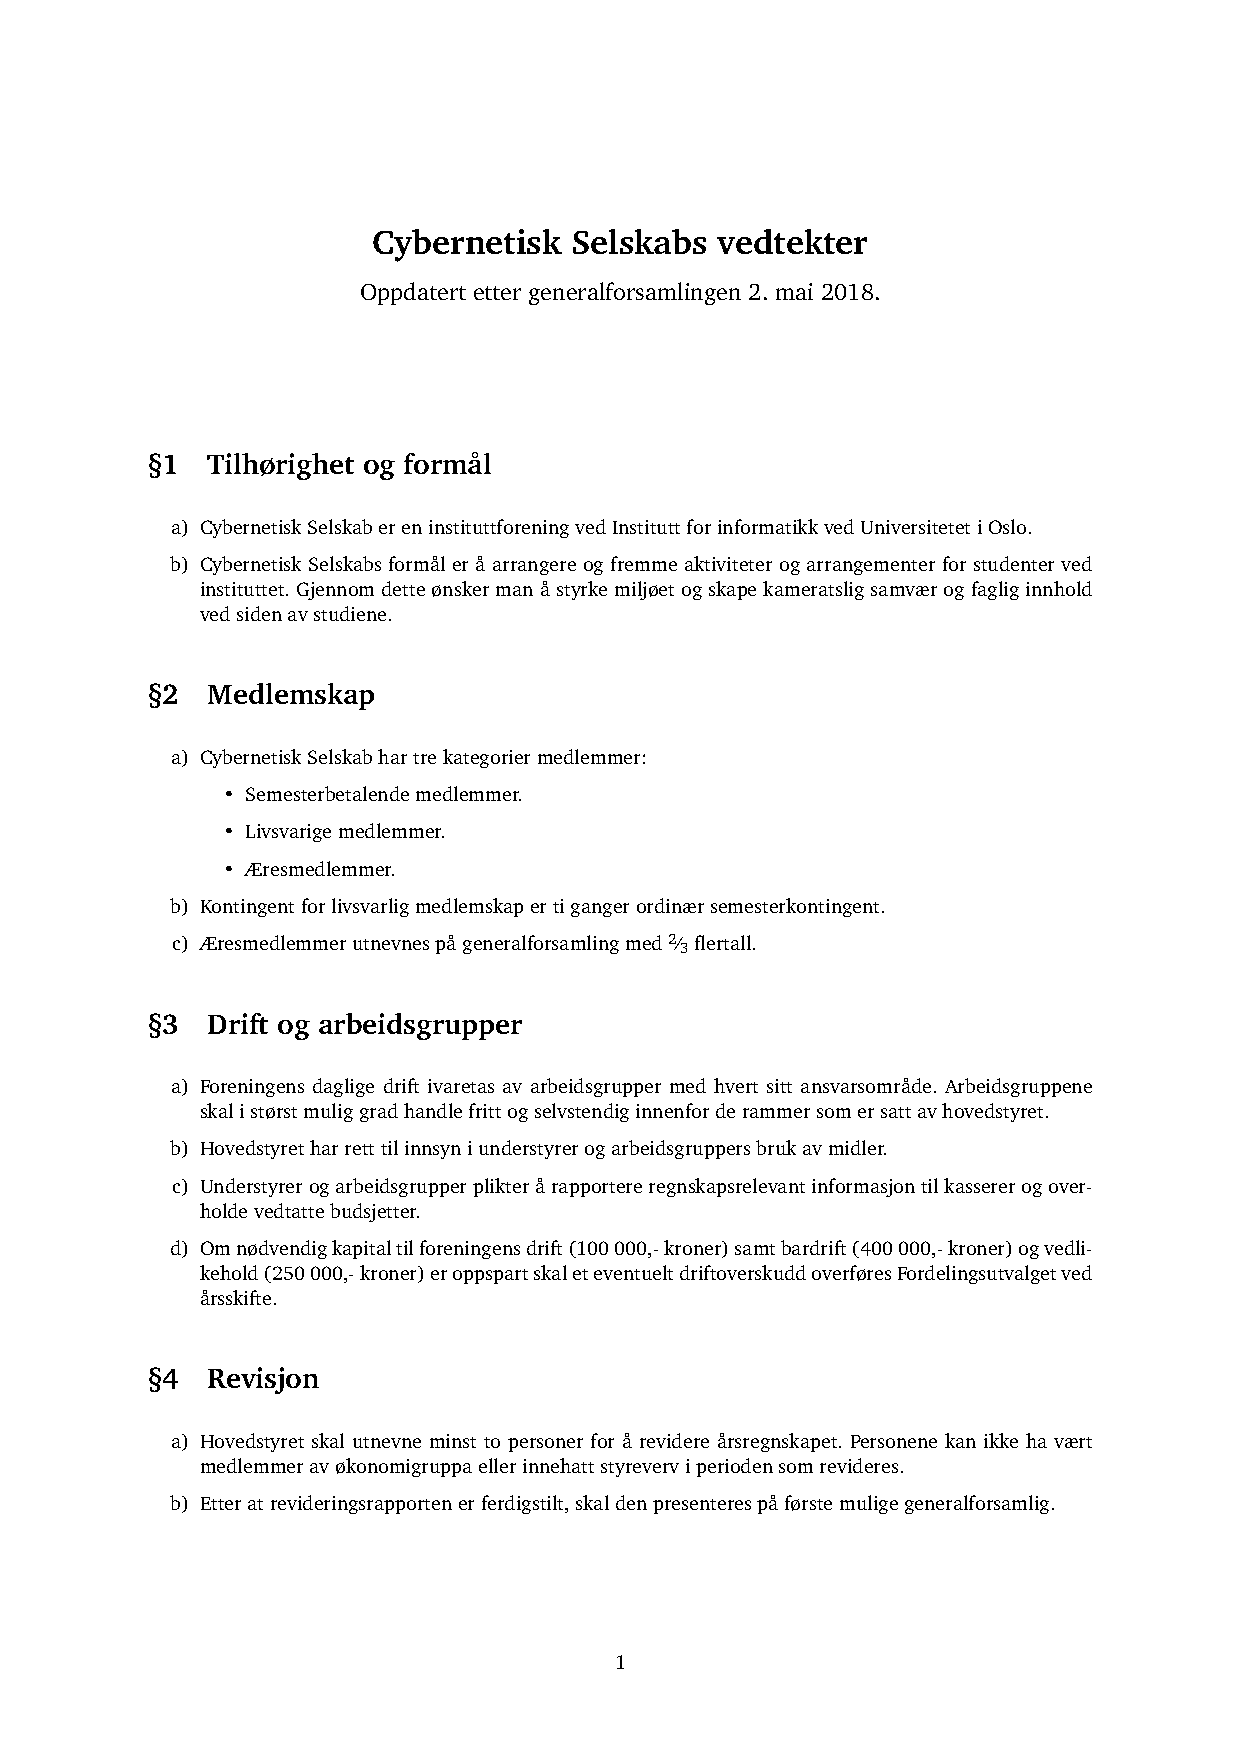
\includepdf[pages=-]{vedtekter.pdf}
\end{document}
